% Options for packages loaded elsewhere
\PassOptionsToPackage{unicode}{hyperref}
\PassOptionsToPackage{hyphens}{url}
\PassOptionsToPackage{dvipsnames,svgnames*,x11names*}{xcolor}
%
\documentclass[
  openany]{book}
\usepackage{lmodern}
\usepackage{amssymb,amsmath}
\usepackage{ifxetex,ifluatex}
\ifnum 0\ifxetex 1\fi\ifluatex 1\fi=0 % if pdftex
  \usepackage[T1]{fontenc}
  \usepackage[utf8]{inputenc}
  \usepackage{textcomp} % provide euro and other symbols
\else % if luatex or xetex
  \usepackage{unicode-math}
  \defaultfontfeatures{Scale=MatchLowercase}
  \defaultfontfeatures[\rmfamily]{Ligatures=TeX,Scale=1}
\fi
% Use upquote if available, for straight quotes in verbatim environments
\IfFileExists{upquote.sty}{\usepackage{upquote}}{}
\IfFileExists{microtype.sty}{% use microtype if available
  \usepackage[]{microtype}
  \UseMicrotypeSet[protrusion]{basicmath} % disable protrusion for tt fonts
}{}
\makeatletter
\@ifundefined{KOMAClassName}{% if non-KOMA class
  \IfFileExists{parskip.sty}{%
    \usepackage{parskip}
  }{% else
    \setlength{\parindent}{0pt}
    \setlength{\parskip}{6pt plus 2pt minus 1pt}}
}{% if KOMA class
  \KOMAoptions{parskip=half}}
\makeatother
\usepackage{xcolor}
\IfFileExists{xurl.sty}{\usepackage{xurl}}{} % add URL line breaks if available
\IfFileExists{bookmark.sty}{\usepackage{bookmark}}{\usepackage{hyperref}}
\hypersetup{
  pdftitle={Data science for the liberal arts},
  pdfauthor={Kevin Lanning},
  colorlinks=true,
  linkcolor=Maroon,
  filecolor=Maroon,
  citecolor=Blue,
  urlcolor=blue,
  pdfcreator={LaTeX via pandoc}}
\urlstyle{same} % disable monospaced font for URLs
\usepackage{longtable,booktabs}
% Correct order of tables after \paragraph or \subparagraph
\usepackage{etoolbox}
\makeatletter
\patchcmd\longtable{\par}{\if@noskipsec\mbox{}\fi\par}{}{}
\makeatother
% Allow footnotes in longtable head/foot
\IfFileExists{footnotehyper.sty}{\usepackage{footnotehyper}}{\usepackage{footnote}}
\makesavenoteenv{longtable}
\usepackage{graphicx}
\makeatletter
\def\maxwidth{\ifdim\Gin@nat@width>\linewidth\linewidth\else\Gin@nat@width\fi}
\def\maxheight{\ifdim\Gin@nat@height>\textheight\textheight\else\Gin@nat@height\fi}
\makeatother
% Scale images if necessary, so that they will not overflow the page
% margins by default, and it is still possible to overwrite the defaults
% using explicit options in \includegraphics[width, height, ...]{}
\setkeys{Gin}{width=\maxwidth,height=\maxheight,keepaspectratio}
% Set default figure placement to htbp
\makeatletter
\def\fps@figure{htbp}
\makeatother
\usepackage[normalem]{ulem}
% Avoid problems with \sout in headers with hyperref
\pdfstringdefDisableCommands{\renewcommand{\sout}{}}
\setlength{\emergencystretch}{3em} % prevent overfull lines
\providecommand{\tightlist}{%
  \setlength{\itemsep}{0pt}\setlength{\parskip}{0pt}}
\setcounter{secnumdepth}{5}
\usepackage{booktabs}
\ifluatex
  \usepackage{selnolig}  % disable illegal ligatures
\fi
\usepackage[]{natbib}
\bibliographystyle{apalike}

\title{Data science for the liberal arts}
\author{Kevin Lanning}
\date{2021-01-01}

\begin{document}
\maketitle

{
\hypersetup{linkcolor=}
\setcounter{tocdepth}{1}
\tableofcontents
}
\hypertarget{section}{%
\chapter*{}\label{section}}
\addcontentsline{toc}{chapter}{}

\hypertarget{preface}{%
\chapter*{preface}\label{preface}}
\addcontentsline{toc}{chapter}{preface}

This work-in-progress will ultimately serve as a textbook for introductory undergraduate courses in data sciences. No prior knowledge of computer programming is presumed, though, ideally, students will have had college algebra (or its equivalent) and an introductory course in statistics, methods, or data analysis.

Data science is still a new field of study, and there are multiple approaches to teaching it and to its place in the college curriculum. This book is intended to serve courses such as the \href{https://kevinlanning.github.io/DataSciSpring2020/}{\emph{Introduction to Data Science}} at the Wilkes Honors College of Florida Atlantic University which, in turn, has drawn from data science classes at the universities of \href{https://idc9.github.io/stor390/}{North Carolina}, \href{https://github.com/STAT545-UBC/STAT545-UBC.github.io}{British Columbia}, \href{https://www2.stat.duke.edu/courses/Fall15/sta112.01/}{Duke}, \href{http://www.hcbravo.org/IntroDataSci/calendar/}{Maryland}, \href{http://pages.stat.wisc.edu/~yandell/R_for_data_sciences/syllabus.html}{Wisconsin}, \href{https://github.com/dcl-2017-04/curriculum}{Stanford}, \href{https://byuistats.github.io/M335/syllabus.html}{BYU}, \href{http://datasciencelabs.github.io/}{Harvard}, \href{https://github.com/MUSA-620-Spring-2017/Course-Materials}{Pennsylvania}, and \href{https://github.com/FAUDataScience/stat259}{UC Berkeley} At each of these schools, the Introduction to Data Science appears, to my eyes at least, closer to Statistics than to Computer Science.

But if our approach is closer to statistics than to programming, it is particularly close to statistics in its most applied and pragmatic form. The choice of statistical methods should follow from the data and problem at hand - or, as \citep{loevinger1957} once put it, statistics should be the handmaiden of real-world concerns rather than technology.

This pragmatic focus is driving the growth of data science in industry, and it is reflected in the way data science is taught at still other schools including \href{https://github.com/UC-MACSS/persp-analysis}{Chicago}, \href{https://github.com/jacobeisenstein/gt-css-class}{Georgia Tech}, \href{https://github.com/raviolli77/dataScience-UCSBProjectGroup-Syllabus}{UC Santa Barbara}, \href{http://www.princeton.edu/~mjs3/soc596_f2016/}{Princeton}, \href{https://github.com/rochelleterman/PS239T}{UC Berkeley}, at \href{https://github.com/HertieDataScience/SyllabusAndLectures}{Berlin's Hertie School of Governance}, and in \href{https://github.com/tommeagher/data1-fall2015}{Columbia's School of Journalism}.

\hypertarget{some-features-of-the-text}{%
\section*{some features of the text}\label{some-features-of-the-text}}
\addcontentsline{toc}{section}{some features of the text}

There are a number of different approaches to teaching data science. The present text includes several distinguishing features.

\textbf{R}

In a recent informal survey of introductory data science courses, I saw a pretty even split between those which begin with Python and those which begin with the statistical programming language R. This difference corresponds, very loosely, to the split noted above: Computer science based approaches to data science are frequently grounded in Python, while statistics-based approaches are generally grounded in R. Our course, like those for most of the syllabi and courses linked above, will be based in R.

\textbf{Reproducible science}

The course will provide an introduction to some of the methods and tools of reproducible science. We will consider the replication crisis in the natural and social sciences, and then consider three distinct approaches which serve as partial solutions to the crisis. The first of these is training in a notebook-based approach to writing analyses, reports and projects (using R markdown documents). The second is using public repositories (such as the \href{https://osf.io/}{Open Science Framework} and \href{https://github.com/}{GitHub}) to provide snapshots of projects over time. Finally, the third is to consider the place of significance testing in the age of Big Data, and to provide training in the use of descriptive, exploratory techniques of data analysis.

\textbf{Good visualizations}

Part of Type C data science is communication, and this includes not just writing up results, but also designing data displays that incisively convey the key ideas or features in a flood of data. We'll examine and develop data visualizations such as plots, networks and text clouds. More advanced topics may include maps, interactive displays, and animations.

\sout{\textbf{All}} \textbf{\emph{Some of}} \textbf{the data}

It's been claimed that in the last fifteen years, humans have produced more than 60 times as much information as existed in the entire previous history of humankind. (It sounds like hyperbole, but even if it's off by an order of magnitude it's still amazing). There are plenty of data sources for us to examine, and we'll consider existing datasets from disciplines ranging from literature to economics to public health, with sizes ranging from a few dozen to millions of data points. We will also clean and create new datasets.

\sout{\textbf{All}} \textbf{\emph{A few of}} \textbf{the latest tools}

One feature of Data Science is that it is changing rapidly. The tools, methods, data sources, and ethical concerns that face us in 2021 are different from those which shaped the field just one or two years ago.

In fields that are undergoing rapid change, there is some trade-off between building expertise with existing (older) tools and trying the newer approaches. Partly because I want to equip you with skills which will not be obsolete, partly because some of these new approaches promise more accessibility, elegance, and/or power, and partly because of my own interest in staying current, we'll be using some of the latest packages and programs.

In the last few years, I've shifted the class from the standard R dialect (as I learned it from the \href{https://www.coursera.org/specializations/jhu-data-science}{Johns Hopkins-Coursera Data Science Specialization}) to the Tidyverse. This year, for the first time, most of our work with the R language will take place online, using \href{https://rstudio.cloud/}{RStudio cloud}, for this should help overcome some hiccups that arise when students are using different machines, operating systems, etc., and should facilitate collaboration among us as well. We'll also be experimenting for the first time with the \href{https://rstudio.github.io/learnr/}{learnr} package, and emphasizing other approaches to learning R, including \href{https://swirlstats.com/}{Swirl} less.

In the past, I've used the Slack platform for messaging, communication and collaboration; this year, I've somewhat reluctantly moved to the Canvas LMS. And, in the past, I've recommended using dedicated markdown editors such as \href{https://typora.io/}{Typora}. While I still think that these are great for some text-editing and note-taking, we'll do our work instead with the editor in the latest variant of RStudio on our laptops, as this allows WYSIWIG (what you see is what you get) formatting of documents - such as this one - that are intended as ``publication-ready'' texts.

We'll continue to use spreadsheets such as Excel or Google Sheets as well.

\hypertarget{the-book-is-for-you}{%
\section*{the book is for you}\label{the-book-is-for-you}}
\addcontentsline{toc}{section}{the book is for you}

It's my intention that this text should serve every college student, regardless of concentration or college major. The skills and insights that you will gain in this course will help you in graduate and professional schools, will help you in your careers, and will help you in your goal of making a better world. And it will help you train the next generation of data scientists as well.

\hypertarget{part-introduction}{%
\part{Introduction}\label{part-introduction}}

\hypertarget{data-science-for-the-liberal-arts}{%
\chapter{data science for the liberal arts}\label{data-science-for-the-liberal-arts}}

Hochster, in \citep{hicks2018}, describes two broad types of data scientists: Type A (Analysis) data scientists, whose skills are like those of an applied \textbf{statistician}, and Type B (Building) data scientists, whose skills lie in problem solving or coding, using the skills of the \textbf{computer scientist}. This view arguably omits a critical component of the field, as data science is driven not just by statistics and computer science, but also by ``domain expertise:''

\begin{figure}
\centering
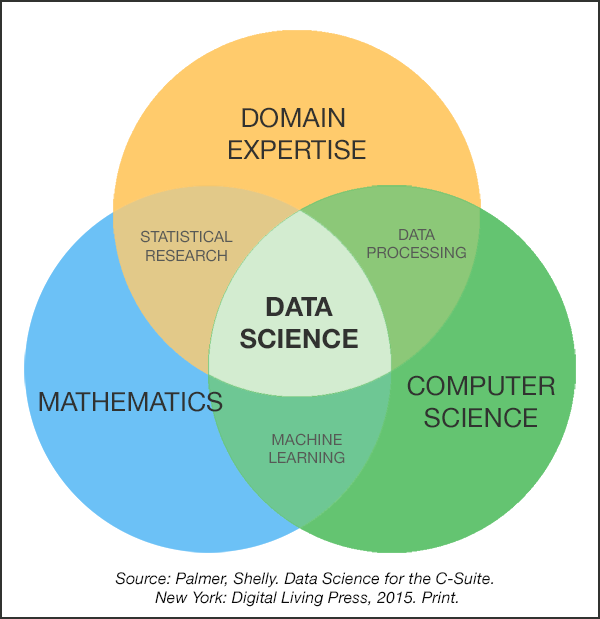
\includegraphics{dataVenn.png}
\caption{\emph{Fig 1.1 - The iconic data science Venn diagram}}
\end{figure}

\hypertarget{type-c-data-science-data-science-for-the-liberal-arts}{%
\section{type C data science = data science for the liberal arts}\label{type-c-data-science-data-science-for-the-liberal-arts}}

The iconic \href{https://www.google.com/search?q=venn+diagram+model+of+data+science\&newwindow=1\&safe=active\&rlz=1C1CHBF_enUS762US763\&tbm=isch\&tbo=u\&source=univ\&sa=X\&ved=0ahUKEwiM_abBtY7XAhXDQCYKHdgyB58QsAQIOg\&biw=1378}{Venn diagram model of data science} shown above suggests what we will call ``Type C data science.'' It begins with ``domain expertise'' in your \textbf{concentration} in the arts, humanities, social and/or natural sciences, it both informs and can be informed by new methods and tools of data analysis, and it includes such things as \textbf{communication} (including writing and the design and display of quantitative data), \textbf{collaboration} (making use of the tools of team science), and \textbf{citizenship} (serving the public good, overcoming the digital divide, furthering social justice, increasing public health, diminishing human suffering, and making the world a more beautiful place). It's shaped, too, by an awareness of the fact that the world and workforce are undergoing massive \textbf{change}: This puts the classic liberal arts focus of ``learning how to learn'' (as opposed to memorization) at center stage. And Type C data science is shaped, not least, by the \textbf{creepiness} of living increasingly in a measured, observed world.

Type C data science does not merely integrate `domain expertise' with statistics and computing, it places content squarely at the center. We can appreciate the compelling logic and power of statistics as well as the elegance of well-written code, but for our purposes these are means to an end. Programming and statistics are tools in the service of social and scientific problems and cultural concerns. Type C data science aims for work which is not merely cool, efficient, or elegant but responsible and meaningful.

\hypertarget{the-incompleteness-of-the-data-science-venn-diagram}{%
\section{the incompleteness of the data science Venn diagram}\label{the-incompleteness-of-the-data-science-venn-diagram}}

Data visualizations are starting points which can provide insights, typically highlighting big truths or effects by obscuring other, presumably smaller ones. The Venn diagram model of data science is no exception: As with other graphs, figures, and maps, it allows us to see by showing only part of the picture. What does it omit? That is, beyond \textbf{statistics}, \textbf{computing/hacking}, and \textbf{domain expertise}, what other skills contribute to the success of the data scientist?

The complexity of data science is such that individuals typically have expertise in some but not all facets of the area. Consequently, problem solving requires \textbf{collaboration}. Collaboration, even more than statistical and technical sophistication, is arguably the most distinctive feature of contemporary scholarship in the natural and social sciences as well as in the private sector \citep{isaacson2014}.

\textbf{Communication} is central to data science because results are inconsequential unless they are recognized, understood, and built upon; facets of communication include oral presentations, written texts and, too, clear data visualizations.

\textbf{Reproducibility} is related to both communication and collaboration. There has been something of a crisis in recent years in the social and natural sciences as many results initially characterized as ``statistically significant'' have been found not to replicate. The reasons for this are multiple and presently contentious, but one path towards better science includes the public sharing of methods and data, ideally before experiments are undertaken. Reproducible methods are a key feature of contemporary data science.

\textbf{Pragmatism} refers to the relevance of work towards real-world goals.

These real-world goals should be informed by \textbf{ethical concerns} including a respect for the privacy and autonomy of our fellow humans.

\hypertarget{a-dimension-of-depth}{%
\section{a dimension of depth}\label{a-dimension-of-depth}}

Cutting across these various facets (statistics, computing, domain expertise, collaboration, communication, reproducibility, pragmatism, and ethics), a second dimension can be articulated. No one of us can excel in all of these domains, rather, we might aim towards goals ranging from \textbf{literacy} (can understand) through \textbf{proficiency} (can get by) to \textbf{fluency} (can practice) to \textbf{leadership} (can create new solutions or methods).

That is, we can think of a \emph{continuum} of knowledge, skills, interests, and goals, ranging from that which characterizes the data \emph{consumer} to the data \emph{citizen} to the data science \emph{contributor.} A Type C data science includes this dimension of `depth' as well.

\hypertarget{google-and-the-liberal-arts}{%
\section{Google and the liberal arts}\label{google-and-the-liberal-arts}}

Data science is at its core empirical, and all of this rhetoric would be meaningless if not grounded in real world findings. Although it was reported in late 2017 that \href{https://www.washingtonpost.com/news/answer-sheet/wp/2017/12/20/the-surprising-thing-google-learned-about-its-employees-and-what-it-means-for-todays-students/?sw_bypass=true\&utm_term=.23e48235d66e}{soft skills rather than STEM training were the most important predictors of success among Google employees}, it's difficult to know whether these results would generalize to a less select group. Nonetheless, there is a clear need for individuals with well-rounded training in the liberal arts in data science positions and, conversely, learning data science is arguably a key part of a contemporary liberal arts education.

\hypertarget{data-sci-and-tmi}{%
\section{data sci and TMI}\label{data-sci-and-tmi}}

One difference between traditional statistics and data science is that the former is typically concerned with making inferences from datasets that are too \emph{small}, while the latter is concerned with extracting a signal from data that is or are too \emph{big} \citep{donoho2017}.

The struggle to extract meaning from a sea of information - of finding needles in haystacks, of finding faint signals in a cacophony of overstimulation - is arguably the question of the age. It is a question we deal with as individuals on a moment-by-moment basis. It is a challenge I face as I wade through the many things that I could include in this class and these notes.

The \emph{primacy of editing} or selection lies at the essence of human perception and the creation of art forms ranging from novels to film. And it is a key challenge that the data scientist faces as well.

\hypertarget{discussion-what-will-you-do-with-data-science}{%
\section{discussion: what will you do with data science?}\label{discussion-what-will-you-do-with-data-science}}

Imagine it is ten years from today. You are working in a cool job (yay). How, ideally, would `data science' inform your professional contributions?

More proximally (closer to today) - what are your own goals for progress in data science, in terms of the model described above?

\hypertarget{references}{%
\chapter{references}\label{references}}

\hypertarget{section-1}{%
\chapter*{}\label{section-1}}
\addcontentsline{toc}{chapter}{}

  \bibliography{references.yaml}

\end{document}
